% The technical aspects have been described very well and a very good understanding is demonstrated. A level of formality has been applied (via accepted design principles, for example) allowing for a concise but thorough description
\chapter{Design and Implementation}
\label{cha:design}
\section{Toolchain}
To develop code for the Hifive1, it was required to develop an effective method of compiling and loading code onto the board, as well as an effective debugger. Initially I used the Sifive's Freedom E SDK with PlatformIO to perform basic prototypes and experiments with the board. However these tools did not provide a sufficient level of control over what was compiled and loaded, as the SDK interacts with many parts of system that were needed for the project, as well as altering the configuration of the board. This meant that the SDK was effective for developing simple applications with the board but did not allow for low level control of operations like iterrupts or privilege levels. Inspection of source code of these lead to useful insights.\\
% https://github.com/riscv-collab/riscv-gnu-toolchain reference?
% To replace these tools I used several applications from the riscv-gnu-toolchain. Used from this was as, with the target architecture of rv32ima\_zicsr\_zifencei, which specifies 32 bit riscv with the standard integer ISA, the multiply-divide extension, the atomics extension, the csr extension, and the fence extension.
% Ld is then used to link the intermediate files. This uses a linker config to specify which sections of the code will be loaded into which sections. This was intitially set to load all parts of the code into RAM, which for the Hifive1 begins at 0x80000000. This was intitially done because at the start of development I wanted to avoid overwriting the pre-loaded double tap bootloader, which enabled the recovery of the board if for some reason a programming error caused a critical fault. However as the project moved on this was no longer possible, as this bootloader interacted with many of the boards configs, which was not acceptable.
% Following this, openocd was used to create a connection to allow GDB to connect with the board.
To replace these tools, I used as and ld from the riscv-gnu-toolchain to assemble and link my code into an elf file that could be loaded onto the board. Also used from that collection was objdump, which was used as a disassembler. The assembler's target architecture was rv32ima\_zicsr\_zifencei, to include all the extensions available on the Hifive1, except for the compressed extension. This was done to prevent the assembler generating a mix of 32 and 16 bit operations, as this causes operations to not be word aligned, and allows jump tables to be implemented without inspecting what instrutions are used. Two linker configurations were used throughout the project, the first which put both the text section and the data section into RAM, whereas the second put text and read-only data in ROM, and left the RAM free. The first configuration was used earlier, as it allowed for safe experimentation with the board while maintaining Sifive's double-tap bootloader. The double-tap bootloader allows normal operation on a regular reset but allows the board to be loaded into a safe mode when the reset is `double tapped', which loads the board into a safe and known state, so that if the board becomes otherwise inoperable it is still able to be recovered. While this was a usefule feature, it limited development, as it also performed several unwanted functions, such as changing the clock configuration, and the uart configuration, which was not acceptable. The second linker config replaced the bootloader in the flash memory with the project code. This was also nessecary as it was not practical to store code in RAM, as it was incredibly limited in space, so the RAM was reserved for program data.\\
To load, run and debug code on the board, I used openocd and gdb. Openocd was used to create an interface with the board, and to specify how the board should be initialized and loaded, and gdb was used to target the openocd interface, which allowed it to load elf files onto the board, and to run/debug code as normal.
% The end of this is gross
% Steps: Started with platform IO with the sifive e sdk
% Then moved onto riscv gnu toolchain with openocd and gdb to load code only into memory
% Then modified the config to load code into the flash
% Mention the bootloader?
\section{Board Configuration}
On the Hifive1, there are several important configuration options that affect general operation of the board. The most notable of these are the clock settings, as these indicate the frequency of the processor, input and output frequencies, and timer interrupts. 
\subsection{Clock settings}
% INCLUDE CLOCK USE FIGURE
The Hifive1 has 3 clock regions, a high frequency clock, a low frequency clock, and a clock used to drive the JTAG connection. The JTAG driver is constant and only used for debugging through JTAG, so is not relevant here.
\\

\begin{figure}[H]
    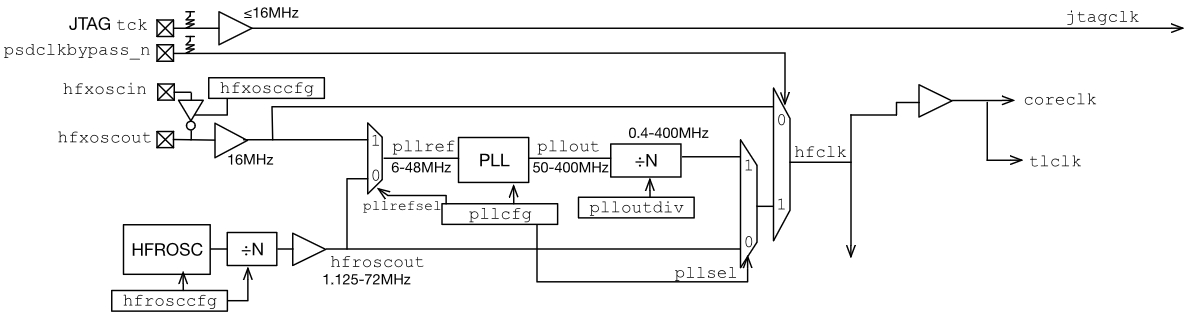
\includegraphics[width=0.9\columnwidth]{figures/hfclock.png}
    \centering
    \caption[High Frequency Clock Diagram]{The high frequency clock generation scheme, specifying how the high frequency clock is driven and configured, taken from the Sifive FE310-G002 Manual\cite{sifive_manual}}
\end{figure}
The high frequency clock controls the processor frequency, and the baud rate of input and output is derived from it. The high frequency clock can be driven from two sources, an internally trimmable high frequency ring oscillator and an external high frequency crystal oscillator. The ring oscillator can produce frequencies ranging form ~1 MHz to 75 MHz, whereas the crystal will produce a constant frequency of 16 MHz. Both of these clock sources may be used `as is', or can be modified using a PLL and divider, giving a available range of 48 MHz to 384 MHz. 
\\
\begin{figure}[H]
    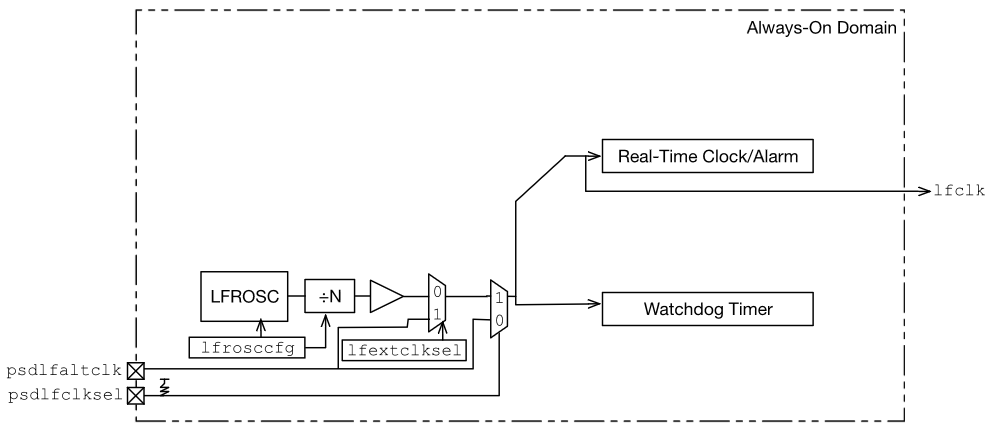
\includegraphics[width=0.9\columnwidth]{figures/lfclock.png}
    \centering
    \caption[Low Frequency Clock Diagram]{The low frequency clock generation scheme, specifying how the low frequency clock is driven and configured\cite{sifive_manual}}
\end{figure}
The low frequency clock is part of the Hifive1 `always on block' and controls the watchdog timer, which can be used to cause a reset on malfunction, and both the real-time clock and the machine timer, both of which are used to generate timed interrupts. Similar to the high frequency clock can be driven from a ring oscillator or from an external clock, which in the Hifive1 is a crystal oscillator. The low frequency ring oscillator functions at 1.5 KHz to 230 KHz using a frequency divider, and the implemented external clock runs at a constant 32.768 KHz, with no option to divide the frequency.
\\
For both clock domains, the crystal oscillator was chosen. The ring oscillator gives the option to operate at a higher frequency, which would result in a higher number of operations per second. While in a practical operating system this would be desirable, since this system is not intended for practical use, a constant frequency was more desirable as it would give more predictable results, and makes \ac{io} operations more reliable. For the low frequency clock, a high frequency would be beneficial for a real time system as the higher frequency would allow for more precise timing of interrupts and other functions, however for an interactive system this precision is not required, and so similar to the high frequency domain the constant frequency of a crystal oscillator was selected.
\section{Traps}
\subsection{Configuration}
There are two methods of implementing a trap handler in \gls{riscv}, direct and vectored. In direct mode, when a trap is called the \ac{pc} is set to whatever value is specified in the upper 30 bits of the MTVEC csr, which is padded to create a 32 bit address. In vectored mode, the synchronous traps are taken identically to direct mode, however asynchronous traps will set the \ac{pc} to the padded value in MTVEC added to four times the trap code. This decreases the number of instructions required before an interrupt can begin exectution. This is useful as it also allows the state of the registers to be preserved, so when a process is preempted it avoids the needed to push several registers to the stack to allow the trap handler to determine the trap type.
\section{Processes}
\subsection{Process Structure}
Due to the extremely limited amount of memory available on the Hifive1, the data required to store information on each process has to be structured carefully, else the amount of memory required to store process information would begin to limit the amount of memory available to the processes themselves. In the current implementation, 35 bytes are used to store process information.
\\
One byte each is allocated for a process id, process parent id, process status, and size of a processes text section. For process id and process parent id, only one byte is needed as the Hifive1 does not have the memory to support a large of processes, so a theoretical cap of 256 processes is acceptable. Process status can only take 4 values, so only 2 bits of the byte are used, and the text size byte stores the size as a power of 2, where a process has \(2^n\) words, where \(n\) is the value stored. While some of these values only require bits, they are stored as bytes to keep the structure word aligned. 
\\
One word each is allocated for the processes program counter, text section pointer and address space pointer. Since memory addresses are word length, these cannot be reduced.
\\
The vast majority of the process structure is used storing the 31 general purpose registers. This is required to retain the state of each process in between scheduling. The only option to reduce this would be to limit the amount of registers available to use. Only 31 must be stored as the x0 register is hardwired to zero.
\\
In other systems, information like the processes stack pointer may be stored, however standard RISC-V calling convention specifies x2 to be used as the stack pointer, so separate storing of this information is not required, and allows a process to handle its address space on its own, however on process creation x2 and x3 are initialized as the stack pointer and the global pointer, where the stack pointer points to the bottom of the process address space and the global pointer at the top. This is done to reduce the overhead of processes that use the standard calling convention.
\subsection{Scheduler}
To implement an interactive system, a scheduler will be designed to allow a process run for a limited time, before halting the process, and running another ready process. The time allowed for a process to run is referred to as its quantum. Processes will be scheduled to be ran in a round robin fashion, to allow a fair runtime to each process while maintaining a low overhead. This is implemented using a circular queue, where new and halted processes are added to the end of the queue, and processes to run are taken from the start of the queue.
\section{Memory Management}
% figures, diagram of memory split into address spaces, labeled process 0 to 6 and machine memory

\section{IO}